Een van de oudste manieren om Windows te configureren is via Control Panel\index{control panel} (Configuratiescherm\index{configuratiescherm}). De settings die je via Control Panel kan beheren worden langzaam over gezet naar de Settings app. Ook in Windows 11 zullen er nog settings zijn die je alleen in Control Panel kan beheren. Het advies van Microsoft is om vooral de Settings app te gebruiken en alleen als het niet anders kan gebruik te maken van Control Panel.

Om Control panel te openen:
\begin{itemize}
\item Klik op het zoek icoon en zoek op control panel
\item Gebruik de windows-toets + r en run Control Panel
\end{itemize}

\begin{minipage}[t]{\linewidth}
\raggedright
\adjustbox{valign=t}{%
	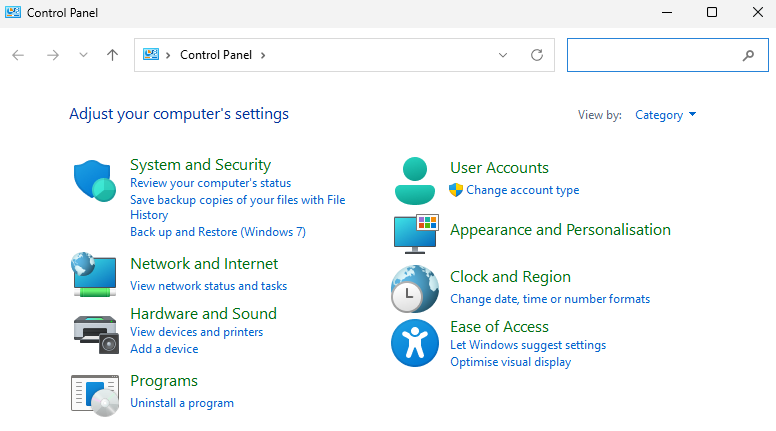
\includegraphics[width=0.99\linewidth]{controlpanel.png}%
}
\end{minipage}

